\chapter{Resultados experimentales: medios de transmisión óptica y acústica}
\label{simulations}
En este capítulo se muestran resultados numéricos y experimentales de la implementación del esquema de seguridad propuesto, para los diferentes módulos y el sistema completo, en medios de transmisión ópticos y acústicos. 
\section{Implementación en software}
Como paso previo a realizar las implementaciones sobre FPGA en el caso óptico, y sobre software en el caso acústico, se implementaron simuladores numéricos de todas las etapas, y se combinaron para comparar los resultados con los teóricos. El simulador fue programado utilizando el lenguaje de C/C++. Fue necesario utilizar este tipo de lenguaje de alto rendimiento debido a que se necesitan simular grandes cantidades de datos para realizar mediciones de tasas de error del orden de 10e-8. Específicamente, en cada paso de simulación se transmite más de 1 Gb de datos por cliente, con hasta 128 clientes, por lo que se requiere del mayor rendimiento posible para obtener tiempos de ejecución aceptables.

\subsection{Estructura general}

La estructura general del simulador es modular, con una separación de alto nivel que obedece al diagrama lógico que puede verse en la figura \ref{fig_comstack}.
Cada módulo representa una etapa en el sistema de comunicaciones que realiza una transformación específica sobre los datos, que puede ser modulación, demodulación, corrección de errores, etc. Los diferentes módulos actúan como filtros, recibiendo y enviando los datos transformados utilizando la entrada y salida estándar del sistema operativo (STDIN/STDOUT). La simulación comienza con un bloque generador de datos binarios aleatorios.

Estos datos son alimentados a la segunda etapa, que es el módulo de corrección de errores. La salida codificada de este módulo es posteriormente alimentada a la siguiente etapa, y de esta manera, los datos originales son sucesivamente transformados en cada módulo.


El medio de transmisión físico es también simulado mediante un modulo que simula las características físicas del canal seleccionado; por ejemplo, en el modulo de simulación óptica, se tienen en cuenta la dispersión y la atención de la señal introducidas por la fibra óptica.

Al llegar a la simulación de la última etapa de la recepción, donde deberían obtenerse los datos originales, el resultado es comparado bit a bit con los datos introducidos originalmente y, en base a las diferencias detectadas, se calcula y reporta el BER. Esta estructura modular brinda flexibilidad al simulador, permitiendo introducir y remover etapas fácilmente.

Sigue a continuación una lista de los módulos y sus características relevantes:

\begin{description} 
 \item[rsenc/rsdec] Codificador/Decodificador de la etapa de corrección de errores. Específicamente, se implementa el algoritmo Reed-Solomon. Es posible generar un código ``recortado'' especificando la cantidad de bytes por bloque en el primer argumento.
 \item[scrambler/descrambler] Implementación del scrambler de datos. El tamaño de bloque puede ser especificado en el primer argumento. Es recomendable que el tamaño de bloque sea un múltiplo del tamaño de bloque del corrector de errores (en nuestro caso, 255 bytes).
 \item[bfenc/bfdec] Etapa codificadora/decodificadora que utiliza el filtro de Bloom. Para simular la interferencia en el medio compartido, en esta etapa se genera un flujo de datos aleatorio por cada cliente a simular y se lo agrega a la trama, lo que provocará colisiones. El único argumento es la cantidad de clientes presentes en el canal.
 \item[noisesim] Simulador de ruido óptico y de distorsión de la señal en la fibra óptica. La tasa de transmisión esta fija a 10 Gb/s. El único parámetro especifica la cantidad de clientes interfiriendo la señal.
 \item[bin2wav/wav2bin] Modulador/Demodulador acústico. Transforma la señal de entrada en ondas acústicas con codificación PCM (\textit{Pulse Coded Modulation}). El módulo de sincronización de audio se encuentra dentro de la utilidad wav2bin.
\end{description}

En general, el simulador puede ejecutar cada etapa consecutivamente, donde cada módulo completará el procesamiento de datos antes de comenzar con la próxima etapa:

\small
\begin{verbatim}
 ./rsenc <${FILE} | ./scrambler ${SCRAMBLEBLOCK} >rs.out
 ./bfenc ${CLIENTES} < rs.out | ./noisesim -c ${CLIENTES} -r 16.6 >bfenc.out
 ./bfdec ${CLIENTES} <bfenc.out >bf.out
 ./descramble ${SCRAMBLEBLOCK} <bf.out | ./rsdec >rsdec.out
\end{verbatim}
\normalsize

En el ejemplo anterior, los módulos utilizan archivos temporales como forma de comunicación. Esto causa que cada módulo deba finalizar el completo procesamiento de los datos de entrada antes de que sean procesados por el módulo siguiente.

Una simple modificación al ejemplo anterior permite prescindir del uso de archivos temporales, mediante la ejecución paralela:
\small
\begin{verbatim}
./rsenc <${FILE} | ./scrambler ${SCRAMBLEBLOCK} | ./bfenc ${CLIENTES} | \
                 ./noisesim -c ${CLIENTES} -r 16.6 | ./bfdec ${CLIENTES} | \ 
                 ./descramble ${SCRAMBLEBLOCK} | ./rsdec > file.out
\end{verbatim}
\normalsize

En la primera configuración del simulador se puede acceder a los archivos temporales intermedios, útiles para depuración y mediciones por etapa, mientras que la segunda configuración tiene la ventaja de aprovechar la totalidad de los procesadores disponibles en el sistema, ya que en un sistema multiprocesador, el sistema operativo usualmente asigna un CPU a cada etapa y estas se ejecutan en paralelo.

La implementación sobre un medio acústico no presenta mayores inconvenientes con respectos a la velocidad de procesamiento, ya que las tasas de transmisión son bajas, acotadas naturalmente por el medio de transmisión y ancho de banda disponible, por lo que los recursos computacionales necesarios para la simulación son limitados. 
Utilizando el medio óptico, normalmente se necesita simular la transmisión de un gigabit o más para obtener una medición confiable del BER del sistema, ya que este medio tiene naturalmente una tasa de transmisión elevada y un BER pequeño, del orden de 10e-12. Adicionalmente, sobre este último medio el sistema soporta un máximo de 128 clientes que son simulados simultáneamente, por lo que los recursos computacionales requeridos son considerables. A raíz de este problema, y aprovechando que la simulación es altamente paralelizable, se implementó un sistema de estilo cliente-servidor donde los cálculos son distribuidos en un grupo de nodos.

\subsection{Etapa de corrección de errores/scrambler}

Los módulos de corrección de errores (rsdec/rsenc) fueron implementados utilizando bibliotecas de código abierto. Se utilizó la popular biblioteca libFEC del autor Phil Karn \cite{libfec}. En cuanto al los módulos de scrambler/descrambler, se implementó un algoritmo de scrambling que utiliza una matriz de permutación aleatoria generada mediante una semilla en cada ejecución, garantizando que las permutaciones sean reversibles.

\subsection{Implementación de filtro de Bloom}
El módulo bfenc/bfdec realiza la codificación/decodificación por software del algoritmo de filtro de Bloom. Los parámetros del algoritmo, tales como el tamaño del filtro $M$ y la cantidad de clientes a simular, son configurables. Una característica que merece mencionarse es la del sistema de minimización de peso de Hamming que es realizado en esta etapa. Tal como se explico en \ref{miniham}, la  implementación se implementó mediante una tabla de lookup (ver tabla \ref{hwtable}), lo que permite consultas muy eficientes con una complejidad temporal de $O(1)$, aunque el tamaño de la tabla (también llamado complejidad espacial del algoritmo) se aproxima a $O(2^{N})$, donde $N$ es la cantidad de bits por símbolo, por lo que para tamaños razonables de $N<24$, la tabla es autogenerada en cada ejecución en función de los parámetros necesarios.

\subsection{Simulador de medio acústico}

El medio de transmisión acústico fue simulado adoptando un modelo físico relativamente sencillo, que sólo toma en cuenta ciertas limitaciones en la respuesta en frecuencia. Para esto, se crearon módulos independientes que realizan la modulación, sincronización, demodulación y filtrado de la señal resultante.
Los módulos transforman los bits de entrada en una señal de audio digital con codificación PCM, a la cual se aplica un filtro pasa banda para simular las limitaciones en frecuencia de los transductores, que comúnmente son son los parlantes y micrófonos de un dispositivo móvil. Este módulo respeta el diseño de los anteriores, emitiendo la señal analógica como un flujo de bytes con codificación PCM vía la salida estándar del sistema. El filtro pasa banda fue implementado como un filtro digital de respuesta finita o FIR \textit{(Finite Impulse Response)}.
Este simulador utiliza algoritmos de modulación, filtros y sincronización reales, por lo que muchos módulos pudieron ser reutilizados sin modificaciones en un medio real. Para más detalles, ver sección \ref{redacus}.

\subsection{Simulador de ruido óptico} 
%% de orte.text

El modelo de simulación del canal óptico toma en cuenta tanto efectos lineales como no lineales en la fibra óptica. 

Se asume que el tráfico proveniente de todas las ONUs alcanza al divisor de $128\times1$ con perfecta sincronización de bit y sin fluctuaciones o \textit{jitter}.
Los casilleros correspondientes al bit `0' contienen una pequeña intensidad óptica de CW (\textit{Continous Wave}, potencia siempre presente en el láser) dada por el razón de extinción de Tx.
Debido a esta potencia óptica siempre presente, cada ONU agregado al sistema agrega una pequeña intensidad de bit `0', incrementando la potencia base total (ver figura \ref{sim:extinction}).
Para la simulación se asume que cada bit `1' agrega un pulso super-Gaussiano ($m=4$) al nivel de potencia base, con un ciclo de trabajo (\textit{duty cycle}) de $1/3$, una aproximación razonable a los parámetros utilizados por el transceptor multigigabit utilizado.

\begin{figure}[!t]
    \centering
      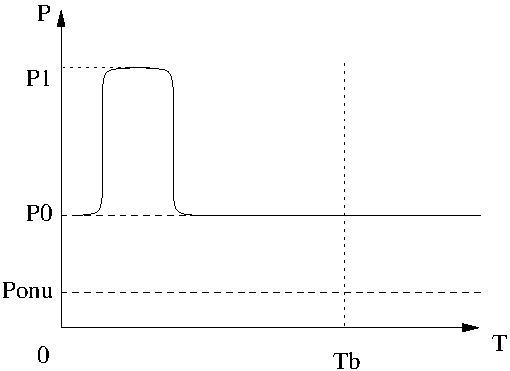
\includegraphics[width=3.5 in]{graphs/extinction.pdf}
      \caption{Diagrama de un bit supergaussiano (m=4) con ciclo útil de 1/4. La potencia del nivel del cero no equivale a potencia cero, sino a $P_0$, que se define como $P_0=P_{ONU}*n$ donde $n$ es la cantidad ONUs activas, y $P_{onu}$ es la potencia generada cuando el láser emite el bit `0'.}
      \label{sim:extinction}
\end{figure}

%The physical optical channel simulation block provides an estimate of
%the BER performance of the optical channel. Simulation steps are as
%follows: RZ upstream traffic coming from all ONUs is assumed to arrive
%at the $128\times1$ splitter with perfect time synchronization, i.e., there is no timing jitter. 
%This allows to simulate merged traffic as a simple addition of optical intensities at bit slots for either `0' or `1' bits. % borrar!
%The `0'-bit slots contain a small CW optical intensity given by the Tx extinction ratio. 
%Each on-line ONU adds its `0'-bit optical intensity yielding a base power level.
% As many bit `0' optical intensities are added as on-line ONUs to produce a base power level.  
%Each `1'-bit adds a super-Gaussian ($m=4$) pulse, duty cycle $1/3$, to the base power level. %, with rising edge at slot start and peak amplitude accordingly to Tx optical mean output power.
% As many bit `1' intensities are added to base level as active Tx there are at each simulation bit slot.

Tanto el tráfico saliente como el entrante sufren atenuaciones debido a múltiples factores que incluyen pérdidas en el divisor, fibra y empalme (\textit{splice}). El presupuesto de potencia (\textit{power budget}) se balancea mediante un EDFA (\textit{erbium-dopped fibre amplifier}) con una ganancia constante de $27$~dB, valor calculado como el necesario para compensar las pérdidas totales sobre un enlace de 10 Km. Un factor en el incremento del BER sobre enlaces ópticos es  la emisión espontánea amplificada del EDFA. Este parámetro es modelado como ruido blanco gaussiano, con una intensidad proporcional a la figura de ruido del amplificador ($7$~dB), y es agregado luego del modelado del EDFA.

%Upstream and downstream merged traffic suffers from attenuation due to
%splitter, fiber, and
%splice losses. The power budget is balanced by an EDFA with $27$~dB constant gain.
%Amplified spontaneous emission from the EDFA is modeled by white Gaussian
%noise, with intensity proportional to the amplifier noise figure ($7$~dB), and is added
%after the EDFA. 

%Real EDFAs gain increases with higher input power, i.e. amplification is not
%linear with number of active Txs. Settling for worst case scenario simulation
%we assume same $27\,dB$ gain for any number of active Txs. ASE noise produced
%at EDFA is modelled as a white Gaussian noise added to the optical signal. An
%EDFA accomplishing the amplification previously discussed ($-25.5\,dBm$ to
%$1.5\,dBm$) would have an output SNR $\geq 60\,dB$ accordingly to a estimation
%based on the bandwidth of forthcoming optical filtering at APD detector (see
%section 6.5.1 at~\cite{Agrawal:xx}). Dispersion compensation regeneration stage
%operation is accounted for by simulating no dispersion effects. Traffic is
%routed back to all ONUs by a 1x128 splitter through another $10\,km$
%fiber,
%amounting to a $27.5\,dB$ attenuation; so for one active Tx input power at each
%Rx would be $-27\,dBm$.

La señal de entrada óptica al receptor es filtrada con un filtro Butterworth de segundo orden y $25$~GHz de ancho de banda, para luego simular su detección asumiendo la respuesta de un dispositivo PD (\textit{photodiode}) estándar (ver sección 4.4.3 de ~\cite{Agrawal:xx}).
Finalmente, para simular el ruido térmico y ruido de disparo o \textit{shot}, se agrega un componente de ruido blanco gaussiano.

%The input optical signal at the receiver is filtered (2nd order low-pass Butterworth filter, $25$~GHz bandwidth) and photodetected assuming a standard PD responsivity (see section 4.4.3 of~\cite{Agrawal:xx}).
%White Gaussian noise accounting for thermal and shot noise is then added
%to the photocurrent, and 
%electrical filtering is applied (2nd order low-pass Butterworth filter, $14$~GHz bandwidth).
%Simulating the decision process a mean of samples around maximum eye opening is compared to a threshold current. 
%Current in case of `1' bits collision is higher than that of a single active Tx, so threshold is established assuming that later case.

%Real EDFAs gain increases with higher input power, i.e., amplification would not be linear with number of active Txs. 
%Settling for worst case scenario simulation we assume same $27\,dB$ gain for any number of active Txs. 
%ASE noise produced at EDFA is modeled as a white Gaussian noise that's added to the electric field. 
%An EDFA accomplishing the amplification previously discussed ($-25.5\,dBm$ to  $1.5\,dBm$) would have an output SNR $\geq 100\,dB$ accordingly to a estimation based on the bandwidth of forthcoming optical filtering at detector (see section 6.5.1 at~\cite{Agrawal:xx}). 
%Effect on traffic of dispersion compensation regeneration stage is accounted by not including in the simulation pulses deformation due to dispersion. 
%Afterwards traffic is routed back to all ONUs by a $1\times128$
%splitter through another $10\,km$ fiber, amounting to a $27.5\,dB$ attenuation arriving to each Rx with $-27\,dB$ for one active Tx.
%
%A concern was if maximum mean total input power allowed at Rx would be surpassed when multiple Tx were simultaneously active. 
%Simulation shown that the occurrence of 15 simultaneously active Tx was a very rare event {\bf <CUANTO??>}. 
%That would amount to $\sim-15\,dBm$ reaching each ONU Rx, well bellow standard commercial Rx overload of $\sim+0.5\,dBm$, that's maximum acceptable mean input power for a BER$<1\,10^{-12}$. 
%
%Rx optical bandwidth is simulated as a low pass filter (2nd order Butterworth as a digital IIR filter~\cite{IIR}, cutoff frequency $25\,GHz$). Afterwards optical traffic is converted into an electrical current. Then to account for thermal and shot noise at a typical APD white Gaussian noise current is added, with an estimated SNR $\simeq 42\,dB$ (see section 4.4.3 at~\cite{Agrawal:xx}). Then electrical filtering is applied (2nd order Butterworth IIR filter, cutoff frequency $6\,GHz$). Detection procedure is performed by comparison to a fixed current threshold. A previous simulation run with the same number of ONUs but with a single active Tx allows to determine the decision threshold at the time of maximum eye diagram opening. Addition of bit `1' amplitudes (collision) produce a current even higher than for a single active Tx, thus this bit slot will be classified as `1' at optical channel simulation output. 
%Media block account for fiber, EDFA and splitters. It attenuates optical trains (splitters and fiber attenuation minus EDFA gain) and also adds white Gaussian noise to the electric field accounting for ASE noise at EDFA. 
% MUCHO, MUY IMPORTANTE: REVISAR CALCULO OSNR (Fn) y verificar que se determina en detector %[VAB]
% ITU recommendation G. 959.1 states that certain interfaces' should operate normally up to $12\,dBm$ mean total input power. In any case if such power is surpassed it would only cause a very short time blinding of Rx affecting a so small amount of bits that wouldn't affect the logical layer ability to correct them.
% receiver overload: max input power for BER<1E-12
%Receiver block simulates Rx behavior. It's optical bandwidth is taken into account by simulating a low pass filtering of incoming traffic (2nd order Butterworth as a digital IIR filter~\cite{IIR}, cutoff frequency $25\,GHz$). Then optical traffic is converted into an electrical current. White Gaussian noise current is added to account for thermal noise at Rx, being it's SNR $\simeq 42\,dB$ accounting for thermal and shot noise at a typical APD detector (see section 4.4.3 at~\cite{Agrawal:xx}). Afterwards another filter simulates detector's linear channel (2nd order Butterworth IIR filter, cutoff frequency $6\,GHz$). Detection procedure is performed by comparison to a fixed current threshold. A previous simulation run with same number of ONUs but with a single active Tx allows to determine the decision threshold at the time of maximum eye diagram opening. Addition of bit `1' amplitudes (collision) produce a current even higher than for a single active Tx, thus this bit slot will be classified as `1' at optical channel simulation output. 


\section{Redes ópticas}
La implementación del sistema sobre redes ópticas fue el objetivo principal de la investigación.
La simulación tuvo un papel muy importante en el desarrollo y pruebas del algoritmo en este medio debido a las elevadas tasas de transmisión involucradas (el transceptor utilizado puede utilizarse a un mínimo de 1 Gbps y máximo de 9.33 Gbps), cuya observación y medición directa no es sencilla. Sin embargo, parámetros tales como el ancho de bit y relación de extinción pueden obtenerse fácilmente mediante el diagrama de ojo de la señal.

\subsection{Simulaciones numéricas}

Podemos citar dos resultados importantes obtenidos mediante las simulaciones numéricas. 
En el primero, detallado en la figura~\ref{sim:optical}, se muestra que la razón de extinción mínima requerida para lograr un BER arbitrario es directamente proporcional al número de ONUs presentes on-line.
Podemos deducir de este gráfico que mientras más ONUs utilicen el sistema, se necesitarán emisores lásers con una razón de extinción mas elevada. Además, con una mayor cantidad de ONUs, se incrementa el BER por problemas físicos: las fluctuaciones de niveles de potencia cercanos al límite de sensibilidad del dispositivo PD tienen un importante efecto en la detección de la señal.
El ruido de shot o disparo es particularmente preocupante ya que es proporcional a la fotocorriente media. En nuestra propuesta, este ruido es más alto que en PONs comunes ya que la intensidad del bit `0' de todas las ONUs presentes contribuyen al mismo.
%Noise fluctuations at power levels near the PD sensitivity limit have an important effect on signal detection. 
%Detection being made at power levels near PD sensitivity is highly sensitive to changes in noise.
%Shot noise is of particular concern as it is proportional to the mean photocurrent.
%In our network proposal the later is higher than in PONs as bit
%`0' optical intensities from all ONUs are added.
%The resulting base-level optical intensity is then heavily dependent on the Tx extinction ratio.
%Fig.~\ref{sim:optical} shows minimal extinction ratios required to
%achieve an arbitrary BER in the physical layer as a function of the
%number of on-line ONUs.
\begin{figure}[!t]
    \centering
      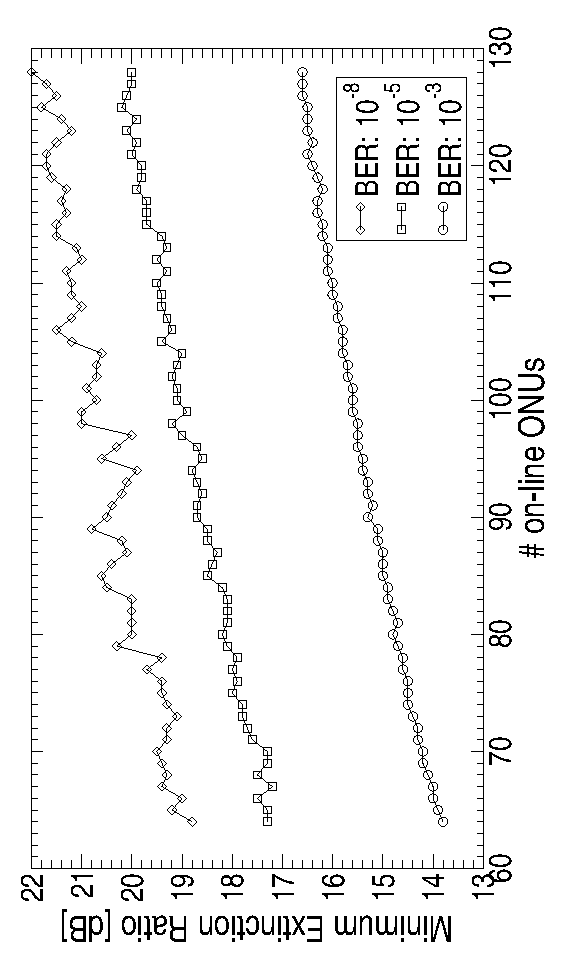
\includegraphics[angle= 270, width=6 in]{graphs/orte03.pdf}
%      \caption{Physical layer simulation result: Minimal extinction ratio required to assure a given BER}
      \caption{Resultado de simulaciones de la capa física: razón de extinción mínima requerida para asegurar un cierto BER.}
      \label{sim:optical}
\end{figure}
En el escenario de $128$ ONUs presentes, un BER menor a 10e-3 puede ser logrado utilizando transmisores del tipo comercial con una razón de extinción de $\simeq16.6$~dB.
Este BER es lo suficientemente bajo para permitir rutinas de corrección de errores al nivel del canal lógico, que garanticen la transmisión libre de errores con una utilización acotada de la capacidad total del canal.
%In the $128$ ONUs scenario a  BER$<10^{-3}$ can be achieved using
%commercially available transmitters with an extinction ratio $\simeq16.6$~dB.
%This BER is low enough to allow for logical-channel error-correction routines that guarantee error-free transmission, while still making use of a fair fraction of channel capacity.
% perform correctly and still use a fair fraction of channel capacity.
% Fig.~\ref{sim:optical} shows simulation results for the BER vs OSNR
% for different numbers of ONUs with fixed electrical SNR $\simeq 42$~dB.
% Higher BERs as ONUs number increases due to the higher probability of
% simultaneous bit `1' transmissions (collisions) yielding pulses of
% optical power higher than that of a logical
% `1', generating intersymbol interference. Higher powers generate higher
% currents at Rxs that demand longer times to settle to logical `0' levels after
% filtering. Nevertheless, as
% can be seen in fig.~\ref{sim:optical}, in the worst case scenario (128
% ONUs) the expected OSNR at the EDFA output is enough ($\geq 40$~dB) to
% ensure a BER$<10^{-7}$. In this case simulation shown that the occurrence of
% 15 simultaneously active Tx was a very rare event, so optical power at Rx
% would be $\simeq -15$~dBm, well bellow standard commercial Rx overload
% of $\sim0.5$~dBm (maximum acceptable mean input power for a
% BER$<10^{-12}$).

\begin{figure}[t]
  \centering
  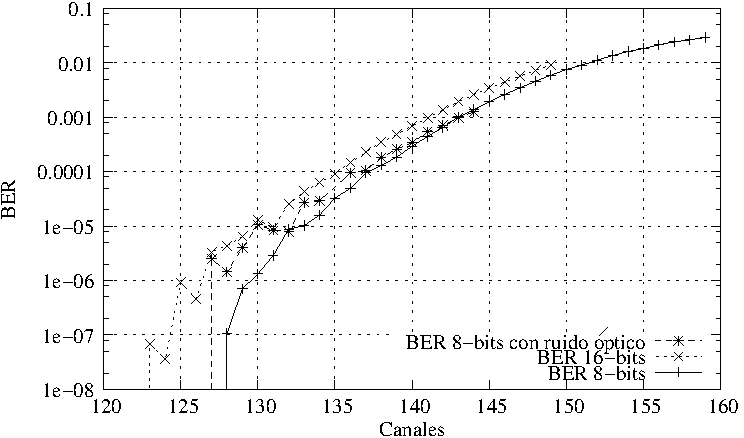
\includegraphics[width=5in]{graphs/BER-tesis.pdf} 
  \caption{BER del canal de un ONU a 10 Gbps vs. la cantidad de ONUs activos. La curva de ``BER 16 bits'' utiliza símbolos de 16-bits. Tiene mejor performance que la curva ``BER 8 bits'' con símbolos de 8 bits. Finalmente, si simulamos el ruido óptico del canal, la performance disminuye ligeramente como puede verse en la curva ``BER 8 bits con ruido óptico''.}
  \label{sim:access}
\end{figure}


La figura~\ref{sim:access} muestra los resultados de la simulación del canal, comparando el BER de un ONU con respecto al número total de ONUs activos. Las dos primeras gráficas muestran la diferencia en rendimiento al utilizar símbolos de 8 bits con respecto a símbolos de 16 bits y, en la tercera gráfica se aprecia el aumento en el BER como resultado de agregar una etapa de ruido óptico a la simulación.
Los resultados fueron obtenidos enviando exactamente un gigabit de datos por cada ONU simultáneamente. El mismo método se utilizó para realizar las simulaciones cuyo resultados se presentan en la figura~\ref{BERvsExpansion}, donde se observa una mejora de rendimiento importante al utilizar el algoritmo de reducción de peso de Hamming.
Volviendo a la figura~\ref{sim:access}, puede verse que cuando la cantidad de ONUs supera los 128, el BER se eleva marcadamente.
De la misma figura podemos observar una disminución de la capacidad en aproximadamente $8$ ONUs cuando el ruido de la capa óptica es agregado a la simulación, debido a la razón de extinción y el ruido producido por el EDFA y los PDs.
Finalmente, la carga máxima que soporta el sistema con un BER de 10e-8 es del $90\%$, lo que significa que en una red de 128 clientes, pueden transmitir simultáneamente hasta 119 ONUs.


%Fig.~\ref{sim:access} shows simulation results for the fraction of the total
%capacity and the BER of one channel at the coding level (circles) and 
%including physical layer impairments (squares). 

%These results were obtained by
%sending one Gigabit of data for each ONU simultaneously.
%This figure shows a channel utilization of $15.7\%$ when all of $128$ ONUs
%are transmitting simultaneously, with a BER$<10^{-8}$. 
%From Fig. \ref{arch:fig1} we observe a penalty of $8$ ONUs when
%impairments from the optical layer (mainly extinction ratio and noise from EDFA and PDs) are taken into account.
%Considering that the system was designed to support asynchronous communications (e.g., Ethernet), it is not likely that all the ONUs will transmit simultaneously (e.g., Internet links often operate at most at $90\%$ load); and therefore our system has a BER $<10^{-8}$ for each channel when 119 ONUs are transmitting at a same time ($119/128>0.9$).
%, removing only one ONU re-establish the desired BER. 
%
%It is worth to remark that, even if the optical channel can induce a
%significant number of errors, the access layer has shown to be able to correct a
%very large number of errors (it is based on
%LDPC+Reed-Solomon+Bloom-Filters), as can be seen on the curve with squares
%at fig.~\ref{sim:access}.
%Observe that the high error rates correspond to a
%worst-case scenario when all ONUs are transmitting simultaneously at
%full capacity, and also 
%there is a low penalty due to physical layer impairments.
%Figure~\ref{sim:optical} presents the simulation's BER vs optical OSNR
%for different numbers of ONUs. %[VAB]
%As the number of ONUs increases higher BERs are obtained at the same optical SNR (electrical SNR is fixed at $\simeq 42\,dB$). In particular there is a penalty of about $30\;dB$ for 128 ONUs in comparison to 1 ONU. This is expected as a consequence of the higher probability of simultaneous bit `1' transmissions (collisions) yielding pulses (logical `1's) of different powers (sum of the power of each transmitter). Higher powers demand more time to settle post filtering current to logical `0' levels. If the following bit slot is indeed a logical `0' an erroneous determination is more possible with a higher collision probability. Nevertheless it can be inferred from simulation results that optical channel should not add significantly to the BER for the whole link as the estimated optical SNR of $\geq 100\,dB$ even for the worst case scenario with 128 ONUs present.
% \begin{figure}[!t]
%     \center
% %     \subfigure[Optical channel]{
% %      \label{sim:optical}
%       \includegraphics[scale=0.4]{BERvsSNR_6GHz.pdf}
% %    }
% %    \subfigure[Logical channel]{
% %      \label{sim:access}
%       \includegraphics[scale=0.4]{BERvsONUs.pdf}
% %    }
%     \caption{Simulation results}
%       \label{archfig}
% \end{figure}

\section{Implementación en FPGA}
El estudio de PONs plantea el desafío de generar, transmitir y recibir señales de 10 Gbps en el laboratorio. El costo de estos sistemas suele ser muy elevado. Uno de los objetivos de esta tesis es presentar una alternativa de muy bajo costo basada en la generación y trasmisión de señales ópticas utilizando dispositivos del tipo FPGA.

\begin{figure}[t]
  \centering
    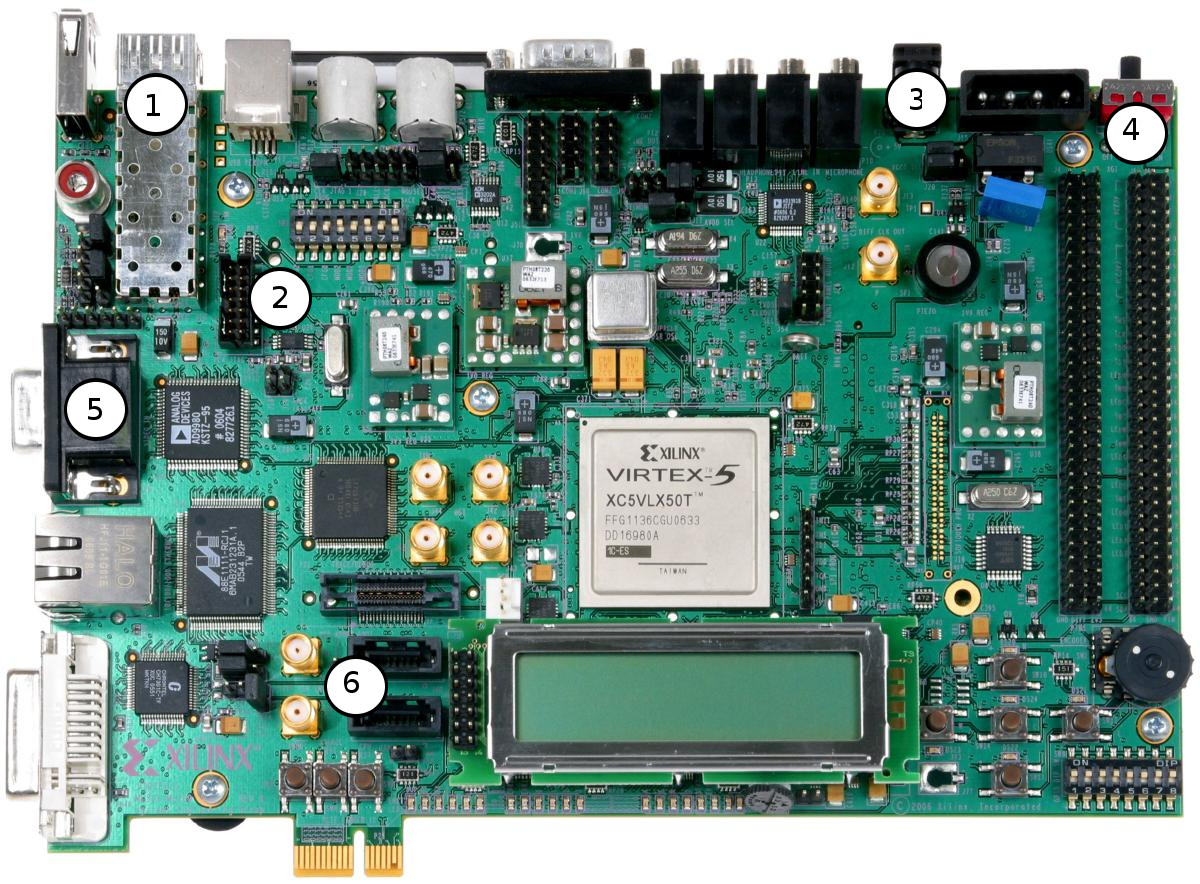
\includegraphics[width=6in]{graphs/ml507.jpg}
\caption {Placa de desarrollo ML570 de Xilinx. Los conectores utilizados son: 1: SFP+, 2: JTAG, 3: alimentación +5V, 4: Switch on/off, 5: Interfaz serial RS232, 6: salida de reloj.}
\label{fig:fpga}
\end{figure}

\subsection{Arquitectura alto nivel de la FPGA Xilinx ML507}
El equipo se compone de un kit de desarrollo ML-507 de Xilinx \cite{virtex5fpga} (ver figura \ref{fig:fpga}) y un transceptor óptico con varios emisores láser con longitudes de onda de 1330 nm y 1550 nm, ambos con capacidad de hasta 10 Gbps en modulación NRZ y alcance de 10km en fibra monomodo \cite{virtex5fpgaRIO}. Para realizar las mediciones se utilizaron dos herramientas de medición:
\begin{itemize}
 \item Osciloscopio óptico Agilent 86100A con módulo óptico 86105A: para
realizar las mediciones físicas contamos con este equipo que posee un
ancho de banda en el módulo óptico de 20 Ghz, suficiente para capturar en
tiempo real los bits individuales o realizar un diagrama de ojo.
\item {\em Integrated Bit Error Rate Tester} (iBERT) \cite{4gtxs}: este dispositivo es un medidor de tasa de error con interfaz para la herramienta de
verificación y depuración ChipScope \cite{arshak2006testing}. Esta herramienta puede denominarse ``virtual'' ya que consiste íntegramente en nucleos IP (\textit{intellectual property}) púramente lógicos, que deben ser sintetizados y embebidos junto con el diseño dentro de la FPGA.
Con iBERT es posible medir en tiempo real varios parámetros del transceptor, así como realizar estadísticas y mediciones de error, variando tasas y características de la transmisión en tiempo real.
 
\end{itemize}
\subsection{Tranceptores multigigabit}
La plataforma de FPGA de Xilinx no fue seleccionada solamente para utilizar la capacidad de procesamiento de la lógica programable para transmisión de datos a altas velocidades, sino por la versatilidad y velocidad de los transceptores multigigabit incluidos en las mismas, esto es, la ``maquinaria'' necesaria para serializar/des-serializar y codificar bits de datos a muy alta velocidad, así como las interfaces para conectar las salidas eléctricas directamente a las entradas de transceptores ópticos, como uno o más SFPs \cite{ug198} (ver figura \ref{fig:fpga}, punto 1). Es necesario mencionar que no existe razón técnica para utilizar un proovedor de FPGAs en particular, ya que muchos proovedores de FPGAs, como por ejemplo Altera \cite{Altera}, venden dispositivos de similares características y precio que Xilinx.

Los transceptores multigigabit están preparados para operar en diversos medios físicos como, por ejemplo, cables trenzados de cobre o líneas de transmisión de alta velocidad sobre PCBs (\textit{printed circuit boards}). Serial-ATA \cite{serial2001high} y PCI-Express \cite{budruk2004pci} son protocolos de transmisión de datos que suelen ser implementados utilizando los transceptores de la FPGA. Sin embargo, en redes de comunicaciones PON, además de funcionar a tasas transmisión  multigigabit se necesitan alcances del orden de kilómetros, características que suelen requerir un medio de transmisión que utiliza fibras ópticas.  El transceptor posee varios módulos adicionales como, por ejemplo, un sistema de sincronización por hardware, sistemas de recuperación de reloj y la capacidad de realizar una codificación 8B/10B \cite{widmer1983dc} adicional, con el objetivo de mantener el balance de DC (\textit{direct current}), pero este último módulo fue desactivado ya que interfiere con los demás codificaciones (para una explicación mas detallada, ver sección \ref{problema8b10b}).

\subsection{Diseño digital del sistema propuesto}
\begin{figure}[t]
  \centering
    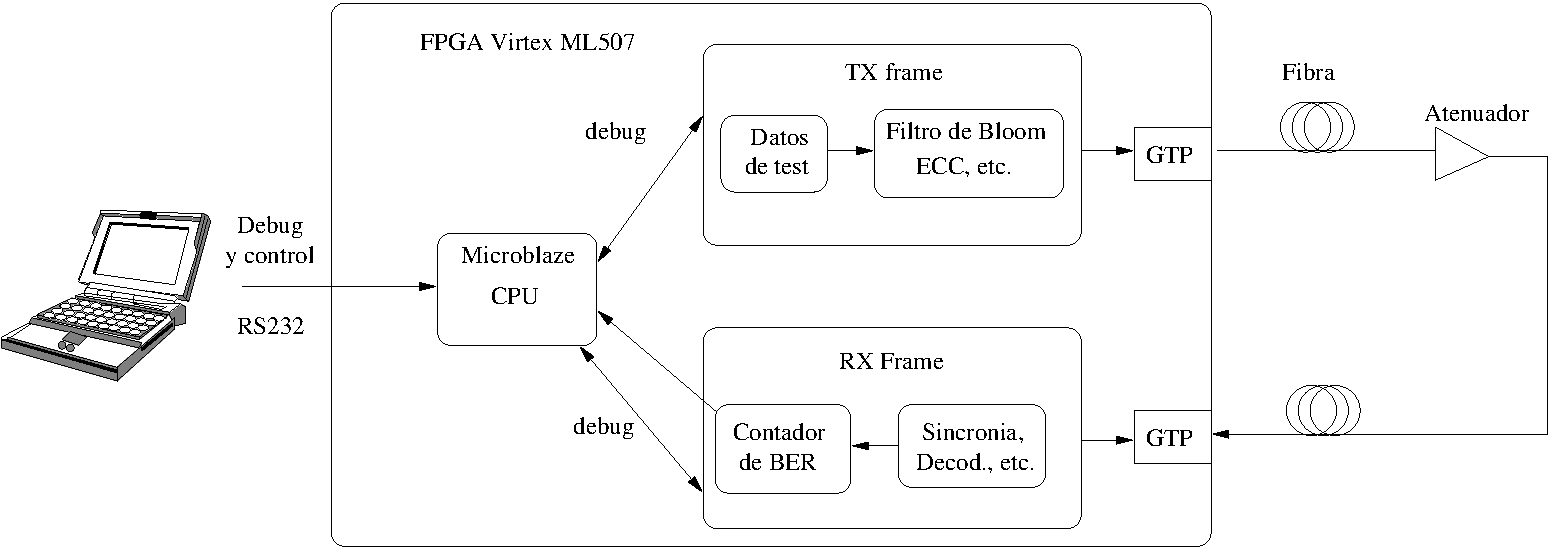
\includegraphics[width=6in]{graphs/fpgadesign.pdf}
\caption {Diseño lógico de alto nivel sobre FPGA}
\label{fig:fpgadesign}
\end{figure}

En la figura~\ref{fig:fpgadesign} puede observarse el diseño digital propuesto en el cual se implementó y probó exitosamente el algoritmo transmitiendo a tasas de 5 Gigabits mediante una fibra óptica.
Estas velocidades fueron logradas gracias a ciertas características del diseño que serán descritas a continuación. En la figura~\ref{fig:fpgahard} se muestra el diseño digital o de hardware. En esta figura, puede verse que el sistema se compone de dos módulos principales: el CPU que actua de módulo de control y el coprocesador de comunicaciones. El diseño fue realizado íntegramente para la Tesis, y puede manejar tasas de 5 Gbps con un reloj del sistema de sólo 75 Mhz.

El módulo de control cumple la función de interfaz entre el sistema y el usuario, permitiendo modificar parámetros de manera sencilla y presentar las estadísticas de una manera rápida. Se presenta al usuario como un sistema de menús en modo texto, mediante los cuales el operador puede ejecutar comandos y leer valores del sistema. La interfaz al usuario se realiza a través de un puerto serial del tipo RS-232. Para su implementación se utilizó un soft-CPU (CPU sintetizado dentro de la misma FPGA) del tipo Xilinx Microblaze \cite{Xilinx:DS865}, y un programa en lenguaje C encargado de imprimir los menús de control y enviar y recibir datos hacia los módulos generadores y decodificadores de trama. Las operaciones se realizan de manera asincrónica con el resto del hardware, por lo que la velocidad de reloj del CPU puede ser muy reducida. Este módulo se implementa en el archivo ``copro1.v'' que también es el módulo principal del diseño, interconectando las señales de todos los submódulos de generación y decodificación de tramas.


\begin{figure}[t]
  \centering
    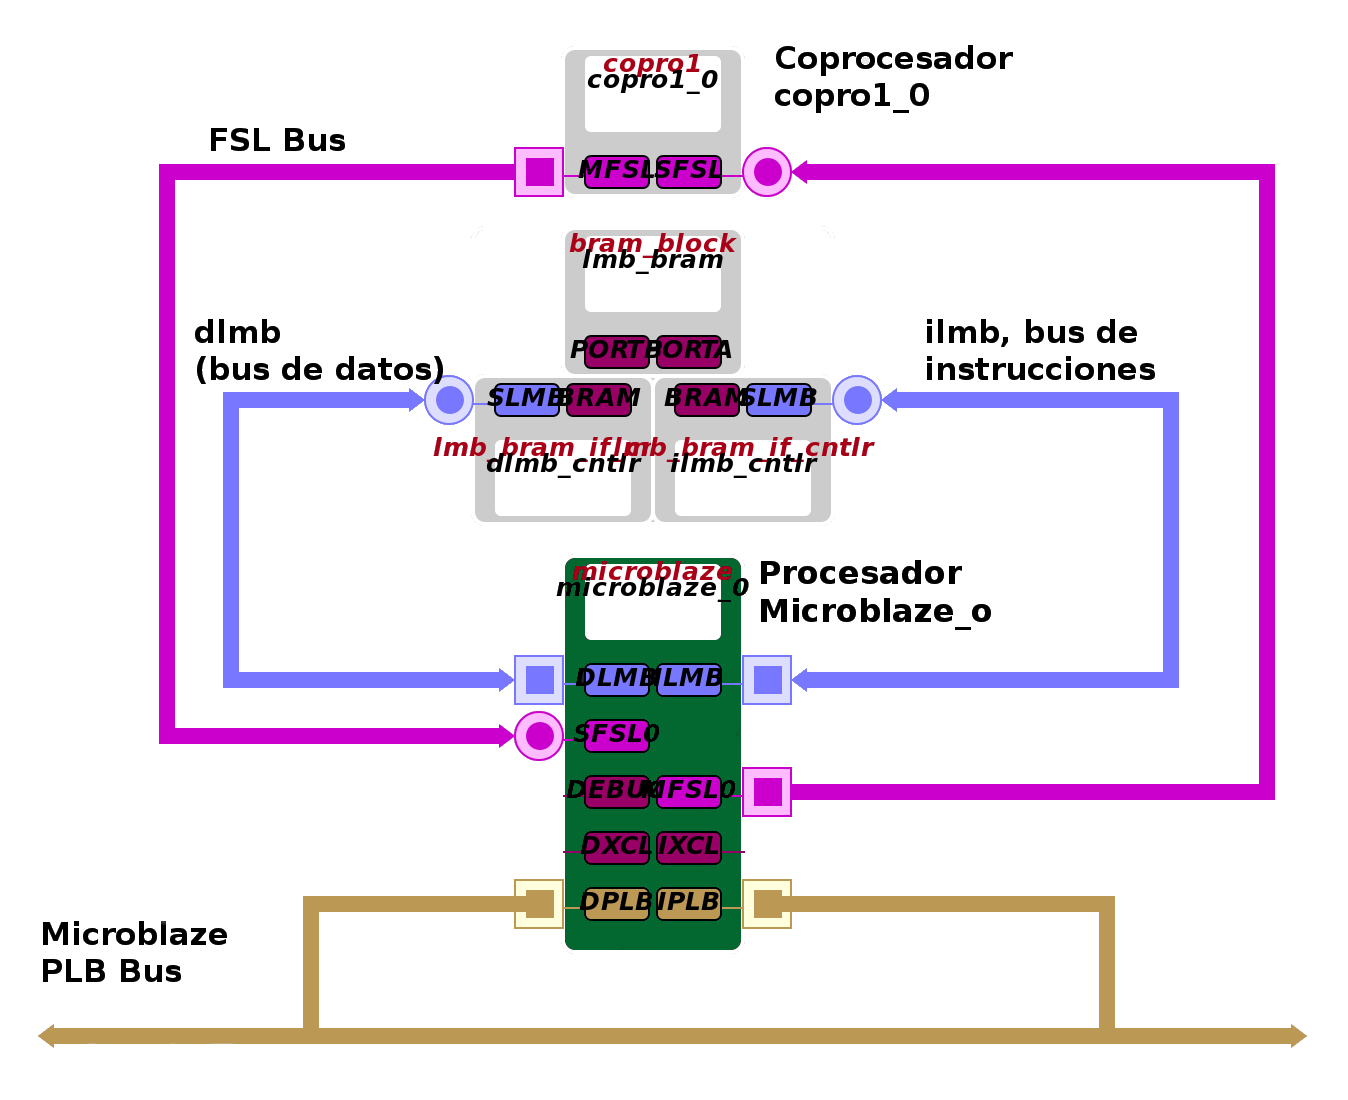
\includegraphics[width=5.25in]{graphs/diagramaXilinx.png}
\caption {Diseño de hardware sobre la FPGA: se aprecian los módulos principales, siendo copro1 el coprocesador de comunicaciones. microblaze\_0 es el CPU y bram\_block es el bloque de memoria utilizado por el CPU, conectado al mismo mediante dos buses: dlmb y ilmb, buses de datos e instrucciones del tipo LMB (\textit{local memory bus}). El coprocesador se conecta mediantes dos buses, llamados copro1\_0\_to\_microblaze\_0 y microblaze\_0\_to\_copro1, ambos buses del tipo FSL (\textit{fast simplex link}). Finalmente, el CPU se conecta a los periféricos como RS232 y switches por medio del bus mb\_plb, del tipo PLB (\textit{peripheral local bus)}.}
\label{fig:fpgahard}
\end{figure}

El coprocesador de comunicaciones puede separarse en cuatro sub-módulos:

\begin{description}
 \item[Transceptor multigigabit:] este componente de hardware es provisto por la FPGA. Puede pensarse en alto nivel como un serializador/deserializador (SERDES), pero contiene más de 15 subsistemas, incluyendo buffers, PLLs (\textit{phase-locked loop}), codificadores y decodificadores. Adicionalmente, el transceptor posee herramientas para sincronización y depuración, permitiendo realizar mediciones y crear lazos de realimentación o \textit{loopbacks} en tres puntos diferentes del flujo de datos para detectar anomalías. Se conecta a la lógica programable de la FPGA por medio de más de 200 señales de control y transferencia de datos, cuyas funciones son encapsuladas por un módulo especial de lógica, que simplifica la interfaz con el resto del sistema. Esta lógica de interfaz se implementó como un módulo de Verilog, llamado ``v5\_gtxwizard\_v1\_7\_tile.v'' en el código fuente.

 \item[Generador de trama:] este módulo se encarga de codificar los datos a transmitir y enviarlos por el transceptor multigigabit. Contiene implementaciones de todas las etapas necesarias, tales como el codificador de ARC4, Bloomfilter encriptado y expansión de peso de Hamming, así como también el sistema de sincronización de trama. La estructura interna es la de una máquina de estados finita, estando implementada íntegramente en lógica digital (sin utilizar ningún componente de software). Se implementó en un sólo módulo de Verilog llamado ``frame\_gen.v''.
 
 \item[Decodificador de trama:] la contrapartida del generador de trama es el decodificador, que posee los decodificadores correspondientes tales como Reed-Solomon, ARC4, Bloomfilter, expansión de peso de Hamming y finalmente el sincronizador de trama, que utiliza parcialmente el hardware de sincronización del transceptor multigigabit para ajustar los tiempos de recepción a nivel de byte, sumado a una sincronización propia para lograr ajustes a nivel de double-word y finalmente, sincronización de la trama (ver sección \ref{fpga:sync}). En lugar de un diseño convencional del tipo CPU+memoria, el diseño de este módulo consiste en una máquina de estados finitos implementada puramente utilizando elementos lógicos de la FPGA. Se implementó en un sólo módulo de Verilog llamado ``frame\_dec.v''. Adicionalmente, un contador de BER se implementó en esta fase, dado que los datos enviados son un patrón de prueba y es posible medir la tasa de errores de manera simple. Las estadísticas de errores son exportadas mediante señales conectadas al módulo de control.
 
 \end{description}

 

El sistema utiliza buffers tanto de lectura como de escritura al transceptor, por lo que puede operar a velocidades de reloj mucho menores. Por ejemplo, si el transceptor multigigabit posee un ancho máximo de bus TXDATAWIDTH y la velocidad de transferencia es TXCLOCK, la velocidad de reloj DATACLOCK necesaria para mantener los buffers internos del transceptor llenos es simplemente $DATACLOCK=TXCLOCK/TXDATAWIDTH$, por lo que transmitiendo a 5 Gbps utilizando el máximo TXDATAWIDTH de 32 bits, tenemos que $DATACLOCK=156Mhz$ un valor alcanzable para la FPGA utilizada y fácilmente implementable en un futuro diseño de ASIC (\textit{application-specific integrated circuit}).
La velocidad de las implementaciones de generador CSPRNG ARC4 y el codificador/decodificador de Reed-Solomon son críticas para la performance del sistema ya que el resto de las etapas no introducen mayores retrasos. El algoritmo ARC4 fue implementado en Verilog poniendo especial énfasis en la performance, logrando un flujo de salida de un byte pseudoaleatorio por cada ciclo de reloj. Para el algoritmo Reed-Solomon se utilizó un IP de la biblioteca de Xilinx que tiene una performance óptima. Exceptuando este último algoritmo de Reed-Solomon, todo el resto del sistema fue implementado desde cero.

% de confEUA.tex

\subsection{Transmisión a 9 Gbps con SFP+}

\begin{figure}[!t]
   \centering
   \subfloat[Tasa de $4.5$ Gbps, 50ns por división.]{{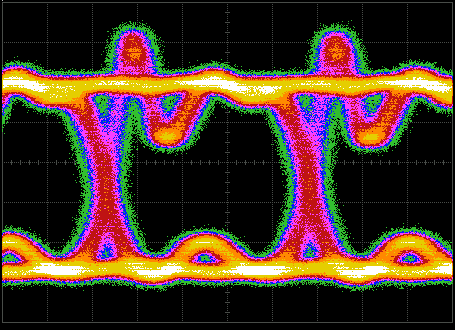
\includegraphics[width=0.45 \textwidth]{graphs/medicionesPaper/eye45G.png} }}%
   \qquad
   \subfloat[Tasa de $7.5$ Gbps, 20ns por división.]{{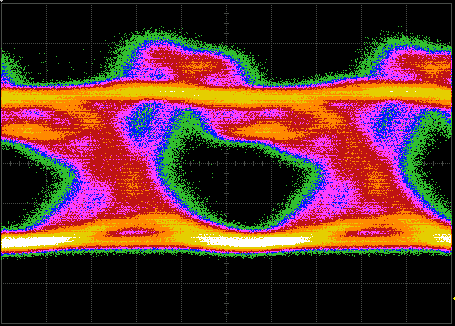
\includegraphics[width=0.45 \textwidth]{graphs/medicionesPaper/eye71G.png} }}%
   \qquad
  \caption {Diagramas de ojo de la señal óptica a la salida de la fibra. Se observa una degradación importante de la calidad de la señal al aumentar la tasa de bits.}
  \label{fig:ImgOjo}
\end{figure}


La norma SFP+ \cite{sff4sff} (\textit{enhanced small form-factor pluggable}) especifica las dimensiones físicas y conectores eléctricos del transceptor óptico. Permite velocidades de hasta 16 Gbit/s y es el formato de transceptor utilizado en la mayoría de los kits de desarrollo de FPGA comerciales actuales.
El transceptor SFP+ consta básicamente de un emisor láser, un detector y circutos ser-des (serializadores/deserializadores).
El montaje para la experiencia se realizó conectando un transceptor SFP+ (ver figura \ref{fig:fpga}, punto 1) con un láser de 1550 nm 
al conector correspondiente en la placa de desarrollo ML-507 y un bucle de
fibra óptica ({\em loopback}), con el objetivo de realizar las mediciones de BER. Adicionalmente, generamos el disparo del
osciloscopio mediante la señal eléctrica de reloj del sistema que
se obtiene a través de los conectores SMA con código J12 y J13 (ver figura \ref{fig:fpga}, punto 6).  
Al disparar el osciloscopio con la señal de reloj sincronizada con la señal de salida, podemos obtener el diagrama de ojo de la señal (ver figura \ref{fig:ImgOjo}).

Para la depuración y configuración se utilizó la interfaz JTAG USB de Xilinx ``Platform Cable
USB II'' \cite{XilJtag} (ver figura \ref{fig:fpga}, punto 2).


\subsection{Configuración del reloj del transceptor}

La tasa de transmisión del transceptor GTX está dada por la
frecuencia de reloj de entrada $F_{PLL\_Clock}$, donde se transmite un
bit por cada semiciclo (la modulación es NRZ); entonces, la tasa de
transmisión será
$R_{line}\mbox{[bps]}=F_{PLL\_Clock}\mbox{[$\frac{1}{s}$]} \times 2$.  La
frecuencia del reloj de entrada del PLL está especificada por la ecuación
5-1 \cite{ug198}:

\begin{equation}
F_{PLL\_Clock} = F_{CLKIN} \times \frac{PLL\_DIVSEL\_FB \times
DIV}{PLL\_DIVSEL\_REF}.% \enspace
\end{equation}\\

donde las constantes $PLL\_DIVSEL\_REF = \{1;2\}$, $DIV = \{4;5\} $ y

$PLL\_DIVSEL\_FB = \{1;2;3;4;5\}$ son configurables por software;
y la frecuencia base del PLL se configura con el switch físico
SW6~\cite[Tabla 1-32]{ug347}.


 Modificando los parámetros puede lograrse, en teoría, un amplio rango
de frecuencias $F_{PLL\_Clock}$, pero de acuerdo a la documentación
del PLL \cite[Pág. 71]{ug366}, este tiene un rango de operación nominal desde $1.2$ a
$2.7$ Ghz. Sin embargo, es posible \cite{OBGAH2010} la
obtención y medición de velocidades de oscilación estables para el PLL
de hasta $4.5$ Ghz (lo que implica una tasa de transmisión de $9$ Gbps),
fuera del rango de operación especificado por el fabricante.

\begin{figure}[t]
  \centering
    %\includegraphics[scale=0.70]{plot.png}
    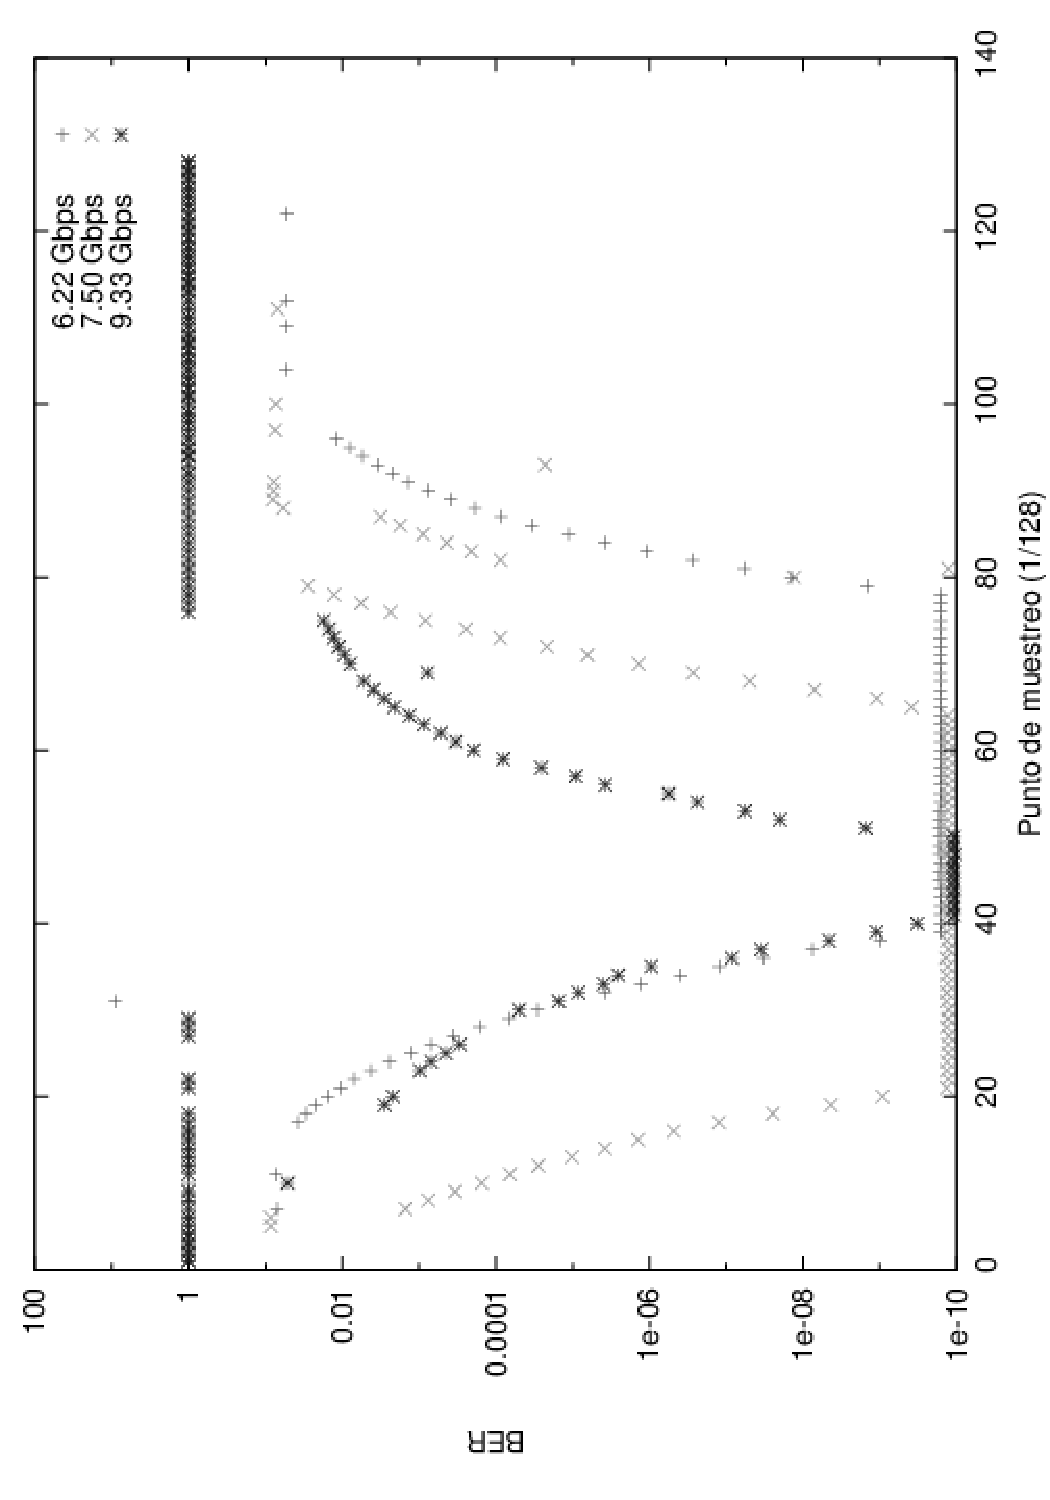
\includegraphics[width=4.2in,angle=270]{graphs/BER_sp_gray.pdf}
\caption {BER vs. punto de muestreo: la FPGA permite muestrear el valor del bit en 128 puntos equidistantes dentro del tiempo de bit. El BER aumenta cuando el punto de muestreo esta cerca de los extremos del bit (valores 0 y 128), donde el diagrama de ojo es más cerrado. Los diagramas de ojo pueden verse en la figura \ref{fig:ImgOjo}.}
\label{fig:BERvsSamplingPoint}
\end{figure}

\subsection{Características del transceptor multigigabit a altas velocidades}


\begin{figure}[!t]
   \centering
   \subfloat[Señal óptica a $4.5$ Gbps]{{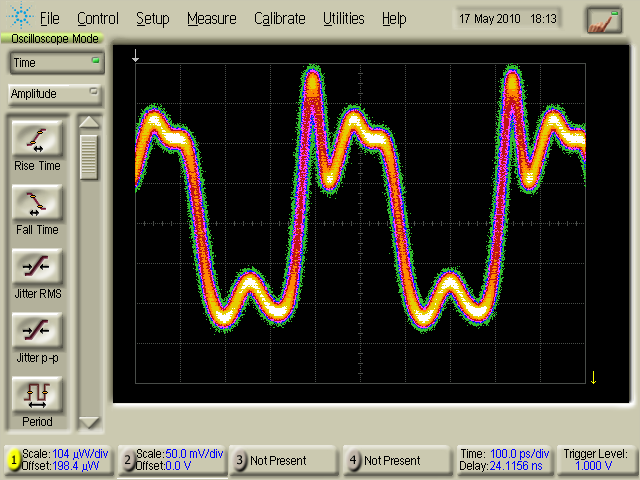
\includegraphics[width=0.40 \textwidth]{graphs/medicionesPaper/screen3.png} }}%
   \qquad
   \subfloat[Señal óptica a $6$ Gbps]{{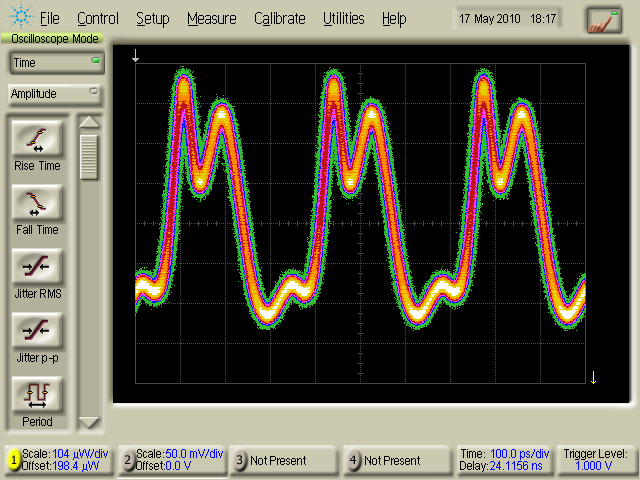
\includegraphics[width=0.40 \textwidth]{graphs/medicionesPaper/screen4.png} }}%
   \qquad
   \subfloat[Señal óptica a $7.5$ Gbps]{{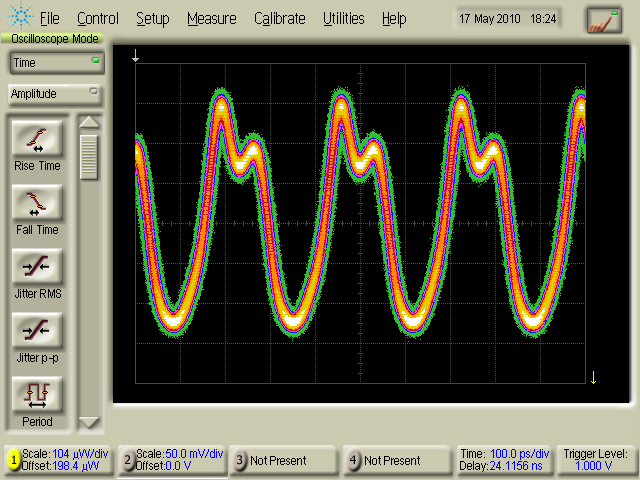
\includegraphics[width=0.40 \textwidth]{graphs/medicionesPaper/screen5.png} }}%
   \qquad
   \subfloat[Señal óptica a $9.33$ Gbps]{{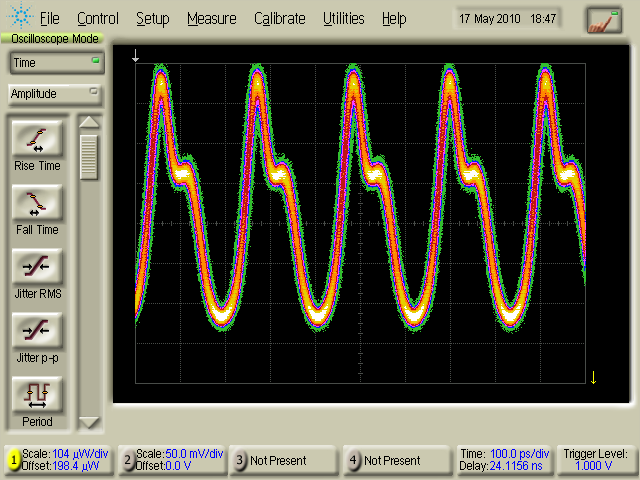
\includegraphics[width=0.40 \textwidth]{graphs/medicionesPaper/screen6.png} }}%
   \qquad
   \subfloat[Señal óptica a $12.44$ Gbps]{{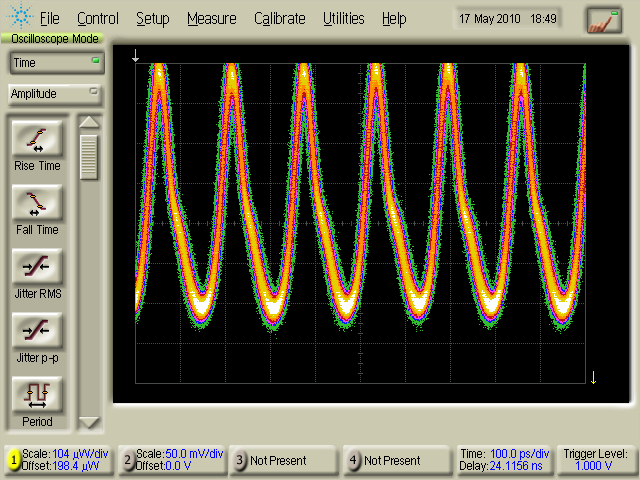
\includegraphics[width=0.40 \textwidth]{graphs/medicionesPaper/screen7.png} }}%
   \qquad
   \subfloat[Señal óptica a $12.44$ Gbps, transmisión 10110101010]{{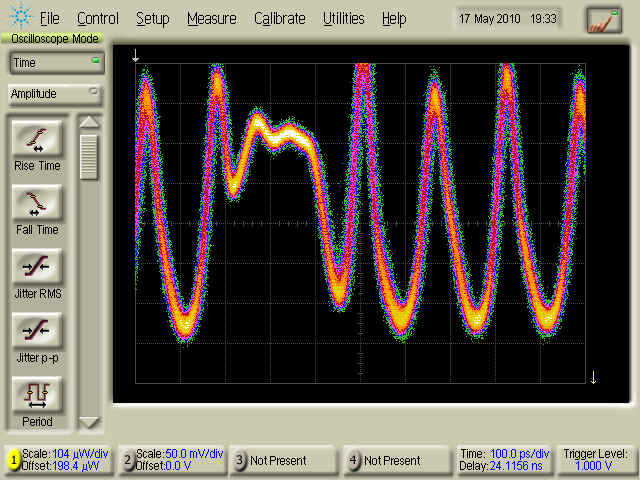
\includegraphics[width=0.40 \textwidth]{graphs/medicionesPaper/screen12.png} }}%
  \caption {Medición de la señal óptica variando la tasa de transmisión de $4.5$ Gbps a $12.44$ Gbps. Se debe tener en cuenta que la señal será distorsionada debido al ancho de banda máximo del módulo de entrada óptico del osciloscopio, que es de 20 Ghz. La secuencia de bits enviada en todas las figuras es ``1010101010'' excepto en la figura f, donde es ``10110101010''.}
  \label{fig:ImgTasa}
\end{figure}





La figura~\ref{fig:ImgTasa} muestra la evolución de la señal óptica producida a diferentes
tasas. Según la documentación del tranceptor \cite{ug198}, la máxima velocidad de transmisión es de $6.5$ Gbps. Sin embargo, en la figura se observan mediciones a tasas mucho mayores, de hasta $12.44$ Gbps. Esto obedece a dos razones:
\begin{itemize}
 \item Es posible transmitir y recibir datos hasta una tasa de 9.33 Gbps, si en lugar de utilizar el procesador de la FPGA para realizar las mediciones, se utiliza el contador interno del transceptor. Esto es, los datos no son generados ni contabilizados por la FPGA, sino por circuitos de testeo dentro del mismo tranceptor, por lo que es posible alcanzar tasas mayores.
 \item Si eliminamos la necesidad de recibir y contabilizar los datos, el transceptor puede generar señales de hasta $12.44$ Gbps. A estas tasas el transceptor sólo puede ser utilizado como un generador de señales, ya que no es posible realizar mediciones de BER. Un estudio más detallado de estos métodos puede verse en \cite{OBGAH2010}.
\end{itemize}


Todas las señales en la figura ~\ref{fig:ImgTasa} corresponden a una transmisión de la secuencia 10101010, excepto la última figura,
que fue generada con una secuencia distinta para demostrar el control sobre la señal generada.

Para determinar el valor del bit, el circuito receptor muestrea la señal de entrada en un punto determinado dentro del casillero o tiempo de bit. Este punto de muestreo de la señal es importante, ya que si se elige correctamente se minimizará el BER, tal como lo muestra la figura~\ref{fig:BERvsSamplingPoint}, donde se aprecia como el BER es minimizado si el punto de muestreo se encuentra aproximadamente en la mitad del tiempo de bit. 
Como puede verse en las figura~\ref{fig:ImgOjo}, a tasas elevadas el pulso del bit se deforma y el punto de muestreo óptimo se modifica.


\subsection{Problema de línea desbalanceada y codificación 8B/10B}
\label{problemacodificacion}
\begin{figure}[t]
  \centering
    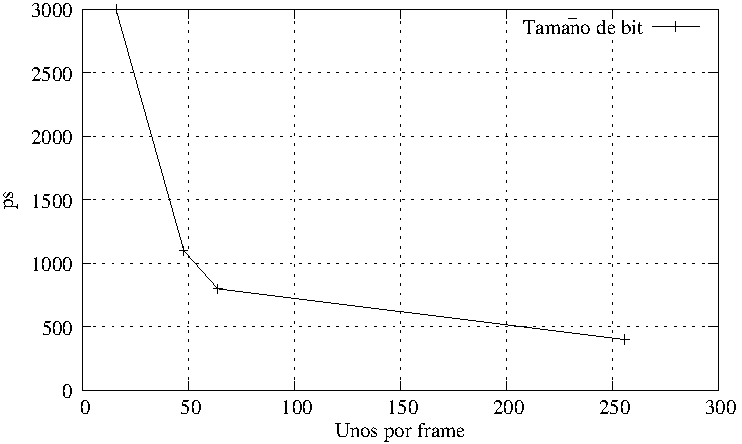
\includegraphics[width=5in]{graphs/expansionbit.pdf}
\caption {Se detalla la expansión del tiempo de bit (en picosegundos) en una señal desbalanceada a medida que la cantidad de unos por trama va disminuyendo. El tamaño de trama es de 512 bits, la tasa nominal es 2.5 Gbps y la duracion del bit es de 400ps.}
\label{fig:expansionbit}
\end{figure}

\label{problema8b10b}
La conexión eléctrica de la FPGA al módulo láser SFP+ se compone de 4 pares diferenciales, que deben transportar señales de hasta 4 GHz. En amplificadores eléctricos de alta velocidad, es deseable que la señal esté balanceada para obtener un componente nulo de corriente continua y poder acotar el ancho de banda necesario. Adicionalmente, una codificación donde se garanticen las transiciones de nivel cada un determinado número de bits, elimina el requerimiento de relojes de alta precisión en ambos lados de la línea de transmisión, ya que el reloj receptor puede re-sincronizarse utilizando dichas transiciones. Esto se logra mediante el denominado circuito de recuperación de reloj.
Uno de estos algoritmos de balanceo es el denominado 8B/10B aunque existen otras codificaciones mas complejas. El transceptor multigigabit de Xilinx tiene un módulo de hardware interno que soporta codificación y decodificación 8B/10B automática de los datos de salida y entrada.

Sin embargo, esta codificación es incompatible con la implementación del algoritmo diseñado sin realizar modificaciones. Si se elimina esta codificación, la señal se degrada tal como se muestra en la figura~\ref{fig:expansionbit}, donde mediante mediciones directas con el osciloscopio óptico se aprecia una expansión progresiva del ancho de bit a medida que el desbalanceo de la señal se hace más pronunciado. Los efectos de la expansión del tamaño de bit son evidentes en la figura~\ref{fig:ImgExpansion} donde las gráficas de potencia óptica ponen en evidencia la expansión e interferencia causada por una señal desbalanceada.
Efectivamente, el receptor recibe hasta 3 ``unos'' por cada ``uno'' transmitido de manera desbalanceada, generando una interferencia que impide el funcionamiento del sistema.


\begin{figure}[!t]
   \centering
   \subfloat[Señal con 256 bits en uno por trama (8B/10B), 400 ps por bit]{{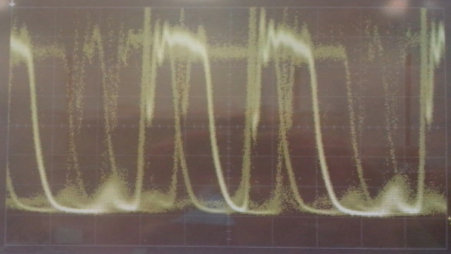
\includegraphics[width=0.45 \textwidth]{graphs/expansion1.jpg} }}%
   \qquad
   \subfloat[Señal con 48 bits en uno por trama, 1100 ps por bit]{{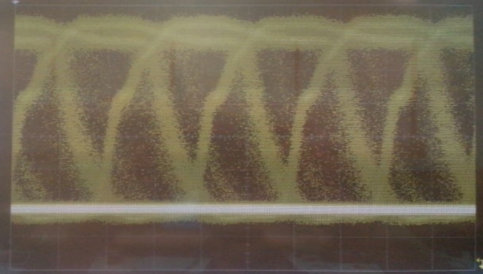
\includegraphics[width=0.45 \textwidth]{graphs/expansion2.jpg} }}%
   \qquad
  \caption {Señal de potencia óptica de un Láser SPF+ Sumitomo de 1330 nm. Se observa una expansión de bit cuando se reduce la cantidad de unos por trama, desbalanceando la señal. La tasa nominal utilizada para estas mediciones es de 2.5 Gbps}
  \label{fig:ImgExpansion}
\end{figure}

Este desbalanceo se soluciona simplemente aplicando las codificaciones a los datos antes de transmitirlos, tales como 8B/10B. Sin embargo, esta transformación es incompatible con el filtro de Bloom, ya que la interferencia de dos señales basta para eliminar la codificación y desbalancear nuevamente la señal. Una posible solución sería utilizar un circuito de transmisión eléctrico compatible con señales desbalanceadas. Para el prototipo se utilizó otra solución, con el objetivo de utilizar la placa ML507 sin modificaciones y poder realizar mediciones sobre el protocolo: en el prototipo, uno de los clientes transmite su señal encriptada normalmente, mientras que los demás clientes son simulados mediante un patrón aleatorio pero balanceado eléctricamente, por lo que la señal es transmitida y recibida correctamente. La señal de estos clientes simulados no puede recuperarse, pero las mediciones son solamente realizadas sobre el cliente real, por lo que el sistema puede funcionar a la máxima tasa soportada por la FPGA (hasta 5 Gbps). El cliente real, al no estar codificado como 8B/10B, introduce un pequeño desbalanceo eléctrico que la línea de transmisión es capaz de soportar sin inconvenientes.

\subsection{Sincronización a nivel de bit, word y trama}
\label{fpga:sync}
\begin{figure}[t]
  \centering
    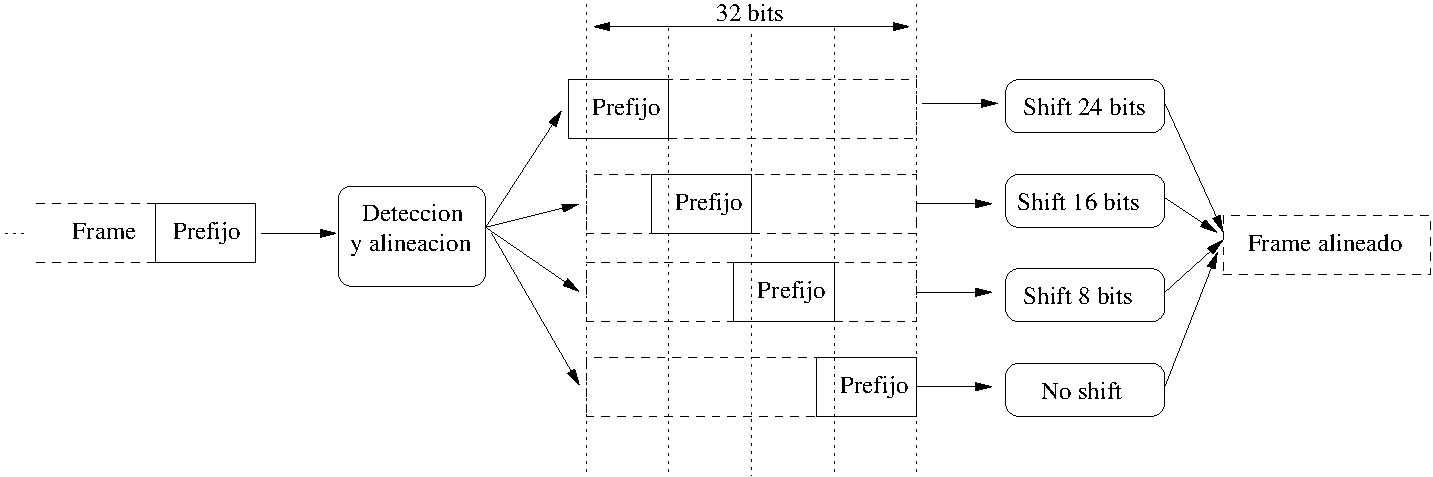
\includegraphics[width=6.2in]{graphs/optsync.pdf}
\caption {Flujo de datos en la sincronización óptica. El mecanismo de sincronización consta de dos etapas: en la primera etapa, el circuito de sincronización de bit alinea la señal entrante al buffer de entrada, colocando el prefijo de sincronización en cuatro posibles alineaciones distintas. La segunda etapa realiza una segunda alineación, detectando la posición del prefijo y utilizando desplazamientos o \textit{shifts} para llevarlo siempre al comienzo del buffer.}
\label{fig:optsync}
\end{figure}


La sincronización no se trató detenidamente en la sección teórica de esta Tesis ya que desde un principio se consideró como un tema ajeno a la misma. Sin embargo, para la implementación final es imprescindible obtener la sincronización entre los nodos que deseen utilizar un canal. Esto no es una tarea sencilla considerando que debe hacerse sobre un canal que contiene una baja relación señal-ruido.

La estrategia utilizada para la transmisión por el medio óptico es utilizar el hardware de sincronización que posee el transceptor multigigabit ya incluido en la FPGA. Este módulo \cite{ug198} denominado ``\textit{Comma Alignment and Detection}'' se basa en la utilización de un prefijo o coma configurable que se compone de una serie de bits (que pueden tener 14 o 20 bits de largo en transceptores de tipo GTX) que se transmite cada vez que se desea sincronizar la etapa RX (receptor) con la TX (transmisor). Esta serie de bits es configurable pero es deseable que posea ciertas características, tales como una alta autocorrelación, para optimizar su detección en el flujo de datos recibidos.
La sincronización se realiza en dos etapas:
\begin{enumerate}
 \item El cliente que desea establecer un canal seguro envía al principio de sus datos el prefijo de sincronización o \textit{comma} (14 bits). Este prefijo es detectado por el módulo de alineación del receptor, que lo coloca en el buffer de entrada. Sin embargo, no se garantiza que el prefijo este siempre al principio del buffer, sino que puede estar tanto en el bit 0 (que sería una alineación perfecta), como en el bit 8, 16 o 24 (Ver figura \ref{fig:optsync}). Esto es debido a que este buffer es de tipo anillo (\textit{ring buffer}).
 \item Una vez alineado el prefijo en el buffer de entrada, se detecta en qué posición ha quedado y comenzar a leer la trama desde la posición siguiente. Esto se realiza en el código Verilog sintetizando cuatro detectores que simultáneamente buscan el prefijo en todas las posiciones posibles y deciden en un sólo ciclo de reloj cuál es la alineación correcta. Al haber sólo 4 posiciones, es un algoritmo eficiente.
\end{enumerate}

En teoría, sólo debería realizarse la sincronización al principio de las comunicaciones. En la práctica, los relojes no son perfectos y es necesario sincronizarlos periódicamente. En la implementación óptica, se envía el prefijo de sincronización al comienzo de cada trama.
Para evitar colisiones, el hardware de alineamiento se desactiva al detectarse una buena sincronización y se reactiva al finalizar la recepción de la trama. Esta es una operación extremadamente rápida, ya que al utilizar una tasa de 5Gbps, cada trama de 1024 bits tiene una duración temporal de 200 ns. Es necesario aclarar que este prefijo adicional no es parte del protocolo de seguridad diseñado y fue implementado como parte del prototipo. Su utilización en la versión final revelaría información útil a un posible atacante, como por ejemplo el comienzo de la trama.

\section{Redes acústicas}
\label{redacus}

Las señales de audio o acústicas resultaron ser un medio de transmisión compatible con el sistema propuesto. Las señales acústicas se interfieren típicamente de manera aditiva y un modem acústico suele representarse como un canal binario simétrico en lugar de un canal Z. Sin embargo, al utilizar ciertas modulaciones, tales como OOK (\textit{on-off Keying}) en donde la frecuencia portadora es varias veces mayor al ancho de bit, existen bajas posibilidades de que la interferencia de dos señales sea destructiva (es decir, que una señal de audio anule a la otra), mientras que los ceros se modulan como silencios y no causan interferencia. Esto puede aproximarse como un canal Z mediante el cual puede implementarse el sistema de comunicación segura descripto en esta Tesis. Debido a las características de modulación necesarias, las velocidades de transmisión son muy bajas, ya que la respuesta en frecuencia de un transductor acústico típico, como un parlante o micrófono, es relativamente reducida, de 2 KHz a 15 KHz, por lo que el ancho de banda disponible es mucho menor con respecto a la implementación óptica.
No obstante, las pruebas e implementaciones sobre este medio pueden ser realizadas totalmente vía software, y el sistema puede ser utilizado en muchas aplicaciones que no requieran elevadas tasas de transmisión pero que requiera privacidad en la comunicación. Ejemplos de aplicaciones de este tipo pueden ser:
\begin{itemize}
 \item Aplicaciones bancarias
 \item Autenticación multi-factor
 \item Compartir datos de contacto sin necesidad de conexión de red.
 \item Compartir URLs
\end{itemize}

La viabilidad de este sistema se demuestra con la reciente publicación de aplicaciones que utilizan este mismo método, utilizando ondas sonoras, para compartir fragmentos de información tales como URLs y contactos. Una aplicación popular de este tipo es Google Tone \cite{GoogleTone}, desarrollada por la empresa Google, que funciona como una extensión de su navegador de Internet.

\subsection{Modulación}
% de newJIS_140512
Las técnicas de modulación en medios de transmisión acústicos son las mismas que pueden utilizarse en medios electromagnéticos.
Sin embargo, no todas las modulaciones siguen el comportamiento de canal Z descripto en la sección \ref{canalZ}.
La modulación OOK (un caso especial de modulación ASK, \textit{amplitude shift keying}), es uno de los tipos de modulación que permite implementar un canal Z sobre un medio acústico si se utiliza sobre cierto rango de parámetros. Utilizando transductores (micrófonos y parlantes) comerciales del tipo presentes en la mayoría de los dispositivos móviles, como por ejemplo teléfonos celulares, la frecuencia de portadora puede variar de 10 kHz a 16 kHz. El mejor rendimiento del sistema se obtuvo con una tasa de transmisión de 1 Kbps al nivel de trama. En las secciones siguientes se detallan las mediciones del retraso (\textit{delay}), el tiempo que le lleva a un bit atravesar la red, que es relativamente elevado debido a una combinación de la baja velocidad de transmisión y la necesidad de un buffer relativamente grande (2048 bits), necesario para la utilización del esquema de corrección de errores seleccionado (Reed-Solomon 223/255). Si bien aumentar la velocidad de transmisión requiere un esfuerzo considerable debido al bajo ancho de banda disponible, la modificación del algoritmo de corrección de errores o sus parámetros (por ejemplo, utilizar algún esquema tipo BCH \cite{bose1960class}) podría reducir el retraso de datos de manera considerable.

Para acotar el ancho de banda de la señal emitida, se utilizó la técnica de ``\textit{pulse-shaping}'', implementada como un filtro FIR \cite{oppenheim1989discrete} (\textit{finite impulse response}) pasa banda a la salida de la etapa de modulación, así como también en la entrada de la etapa de demodulación. Este filtro, además de reducir el ancho de banda utilizado, ayuda a rechazar interferencias.
Adicionalmente, un ciclo de trabajo (\textit{duty cycle}) de 50\% demostró ser el óptimo para la modulación.
%On-Off Keying modulation of sound waves, following the Z-channel interface model described in Section 2.2., encode the transmitted bits as pulses. Carrier frequency can vary from 10 kHz to 16 kHz. Good results can be obtained with a rate of 1000 bps at frame level. In experiments, delay (the time for a bit to traverse the network) was very high, due to Reed-Solomon 223/255 coding, a frame to support up to 16 users and the low capacity of the physical media. A more sensible choice of FEC algorithm (like BCH [12]) could drastically reduce data delay. 

%Simple pulse shaping is realized using a pass-band filter at the output of the modulation and also at the input of the demodulator. This filter also helps reject unwanted interference.
\subsection{Sincronización}
% de newJIS_140512

\begin{figure}[t]
  \centering
    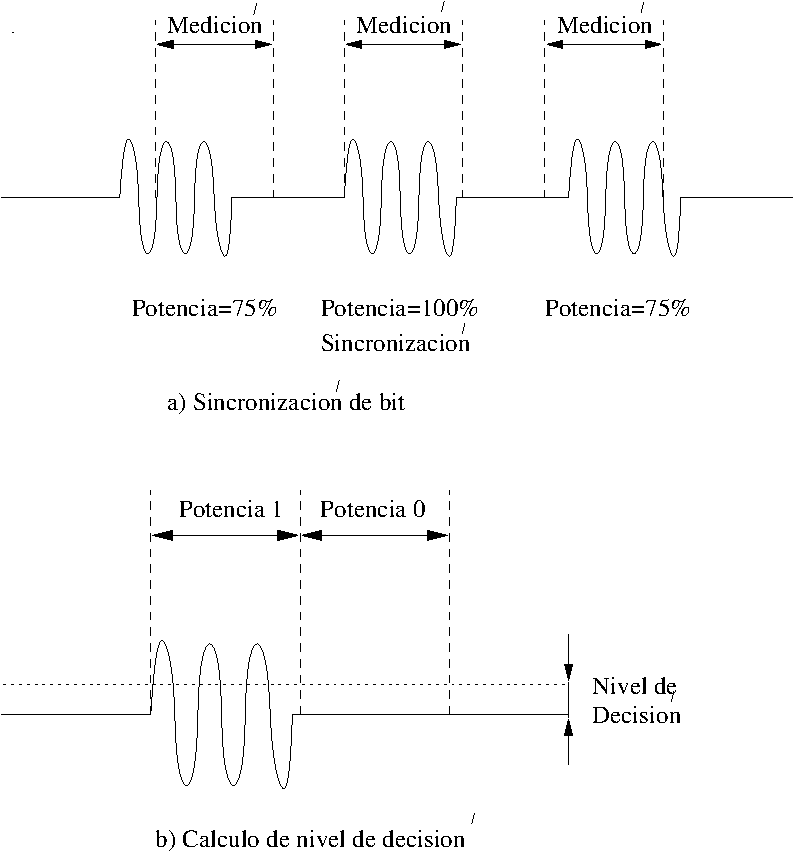
\includegraphics[width=4.5in]{graphs/acusync.pdf}
\caption {Sincronización acústica. En la figura a) se recorren consecutivamente todas las posibilidades hasta encontrar la mayor potencia de bit, que corresponde a la mejor sincronización. Luego, en la figura b) se calcula el umbral de decisión.}
\label{fig:acusync}
\end{figure}

Como se desprende de la descripción del canal de comunicaciones, la sincronización entre el transmisor y el receptor es esencial para la correcta decodificación de la información. 
En el caso del medio óptico, la sincronización de bit y word (16 bits) debe realizarse a tasas tan elevadas que requiere necesariamente soporte de hardware por parte del transceptor.
Sin embargo, las tasas de transmisión de 1 kbps utilizadas en el canal acústico permiten realizar una sincronización por software sin ningún soporte de hardware adicional, al ser una velocidad manejable por cualquier procesador moderno.
El método es muy similar al utilizado en el canal óptico: un patrón inicial de sincronización es enviado para que el receptor pueda realizar un ajuste de parámetros tales como fase y umbral de decisión (ver figura~\ref{fig:acusync}). La deriva y fluctuación del reloj del sistema (\textit{drift y jitter}) no son significativas a esta baja velocidad de transmisión, por lo que no se requiere corrección de ningún tipo, haciendo que la implementación del modem por software sea muy sencilla.
Ciertos parámetros, si bien son inicializados en la etapa de sincronización, son por naturaleza dinámicos y se ajustan periódicamente, como por ejemplo el umbral de decisión, que es recalculado a partir de un promedio de los datos de entrada. La fase es también corregida utilizando los datos de entrada como referencia. Este método de sincronización permite detectar el comienzo de la trama a su vez que se ajusta a nivel de bit; ambas alineaciones son necesarias en cada comunicación (pero la alineación de la trama solamente entre los ONUs comunicantes). Adicionalmente, una vez comenzada la transmisión, los datos serán indescifrables gracias al algoritmo CDMA de \textit{time-hopping} guiado por un CS-PRNG.

%As it follows from the description of the communication channel, synchronization between the transmitter and receiver is essential for the correct decoding of information. For this purpose, an initial synchronization pattern is sent, so the receiver can adjust parameters like phase and decision level (see Figure 3). For the data bits transmission a duty cycle of 50\% showed in our experiments an enhanced detection. Clock drift and jitter are not significant at this low transmission speed and so no correction is required, making the software modem implementation very simple. Decision level is dynamic, meaning it is constantly re-calculated from averaged input data. The receiver symbol phase is also corrected using the input data as reference. Notice that this simple synchronization method allows detecting the frame start as well as the bit slot; both are needed at every communication. Moreover, once the data began to be transmitted, the communication becomes indecipherable thanks to the CS-PRNG.


\subsection{Medición multiusuario}
\begin{figure}[t]
  \centering
    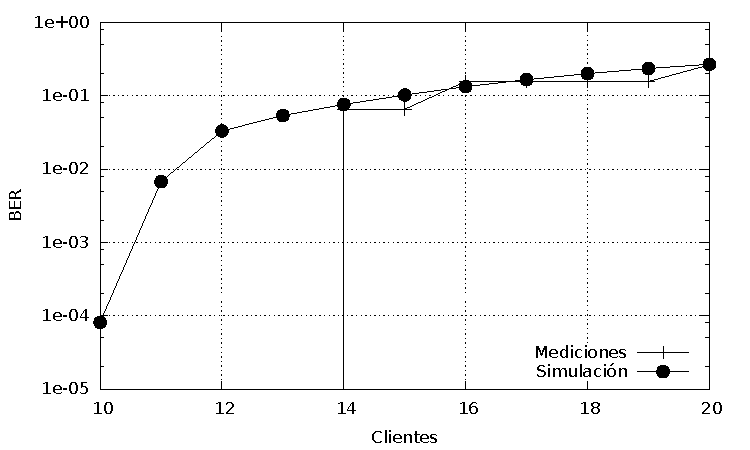
\includegraphics[width=5in]{graphs/medidas_clientes_JIS-fig6.pdf}
\caption {Multi-usuario: BER del enlace entre dos laptops (Lenovo T420 y Lenovo X60), una de ellas simulando varios nodos.}
\label{fig:acumult}
\end{figure}

Todas las mediciones fueron realizadas a una tasa de 1 kbps, utilizando una señal portadora acústica de 16 kHz, que se encuentra en el límite auditivo de la mayoría de las personas adultas \cite{gordon2005hearing}. Es posible que algunos parlantes no respondan correctamente a esta frecuencia, en cuyo caso puede reducirse y utilizar una portadora de 12 kHz. El objetivo de utilizar una frecuencia de audio tan cercana al límite de reproducción de los transductores es incrementar el nivel de confort de los usuarios, que sólo podrán percibir el modem con bajo volumen, o directamente será inaudible. Adicionalmente, las altas frecuencias presentaron menos interferencias de ruido ambiente.
La cantidad total de datos transmitidos por canal fue de 4096 bits en cada medición. El volumen de la señal de salida fue configurado al máximo para cada dispositivo, mientras que la amplificación de la señal obtenida por el micrófono fue optimizada en cada caso para obtener el menor BER.
Con el modulador y circuito de sincronización implementados, el sistema opera con tasas de error aceptables con una separación máxima entre nodos de 1 metro, una distancia que normalmente excede la existente entre un terminal móvil (celular, etc.) y una computadora fija en el mismo escritorio (Ver figura~\ref{fig:acudist}). Aún para un alto número de clientes simultáneos ($> 10$) el sistema no presenta altas tasas de error o ancho de banda reducido, como puede verse en la figura~\ref{fig:acumult}.
En las mediciones, el retraso del canal fue de más de 60 segundos, excesivo para muchas aplicaciones que no necesitan alto ancho de banda pero requieren un corto tiempo de respuesta (por ejemplo, aplicaciones bancarias). El retraso puede ser disminuido de dos maneras: 
\begin{enumerate}
 \item Decrementando la cantidad máxima de clientes simultáneos soportados por el sistema.
 \item Utilizando algoritmos de ECC de bajo retraso y de bloque reducido, tales como BCH, ya que actualmente el retraso se produce en su mayor parte durante la recepción de un bloque completo para el algoritmo de Reed-Solomon (2048 bits).
\end{enumerate}



% De JIS2014MathType.pdf
%All measurements were conducted at a rate of 1000 bps, with the carrier signal at 16 kHz. The total data trans-
%mitted was 4096 bits. Output volume was set at the maximum possible for each device, while the input amplifi-
%cation was optimized for each measurement.
%We measured that the system operates with acceptable error rates for links of up to 1 meter, a distance usually
%exceeding that between a mobile terminal (phone, etc.) and a fixed computer placed in the same desk (see Fig-
%ure 7). Even for a high number of concurrent clients (>10) the system does not present high error rates or re-
%duced bandwidth, as can be seen in Figure 6.
%Although in the present test channel delay was longer than 60 seconds, excessive for some applications re-
%quiring short response time (e.g. banking transactions), this parameter can be reduced by decreasing the maxi-
%mum number of simultaneous users supported by the system and using a lower-delay interleaver and an outer
%error correction algorithm like BCH
%

\subsection{Mediciónes a distintas distancias}

\begin{figure}[t]
  \centering
    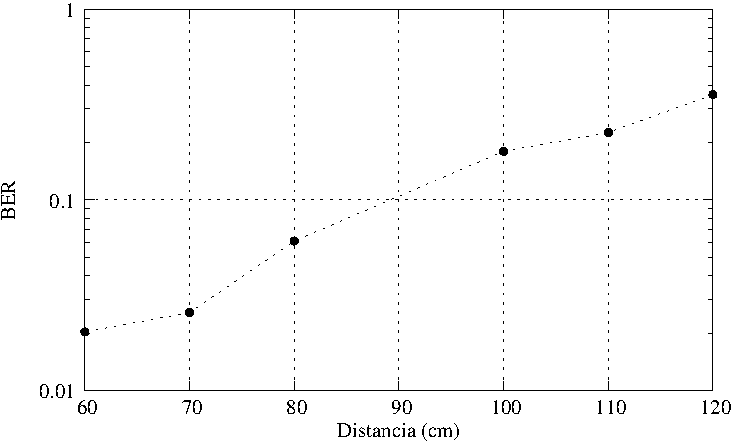
\includegraphics[width=5in]{graphs/mediciones-distancia-fig7.pdf}
\caption {Distancia vs. BER: el enlace acústico entre una Laptop (Lenovo T420) y un celular (HTC Status) presenta errores detectables cuando se superan los 60 cm de separación entre ambos dispositivos.}
\label{fig:acudist}
\end{figure}

Las comunicaciones acústicas utilizando como portadora un tono de 12 kHz son muy susceptibles al ruido ambiente. Un enlace acústico con 50 cm de separación entre una notebook Lenovo T420 y un celular HTC Status (ver figura \ref{fig:acudist}) tuvo un $15\%$ de BER con sólo una ligera interferencia (como por ejemplo, golpear una mesa cercana). Esta observación motivó el uso de la frecuencia más alta posible. Una portadora de 16 kHz presentó el mayor rango de compatibilidad entre los dispositivos, aunque algunos de ellos demostraron no poder emitir audio a frecuencias mayores.
Los parlantes de una Laptop Lenovo T420 y otra Laptop Lenovo X60 fueron capaces de establecer un enlace utilizando como portadora un tono de 19.2 kHz, aunque sólo en cortas distancias (20 cm). De todas formas, esta frecuencia de portadora permitió un mayor ancho de banda en el enlace (2 kbps en lugar de 1 kbps) con la misma tasa de error.
%La señal acústica modulada puede causar molestias a personas o animales cercanos. Distintos tonos de portadora causan distintos efectos y niveles de molestia, aunque este último parámetro es subjetivo. La portadora de 19.2 kHz fue descrita como no audible, mientras que la portadora a 16 kHz y 12 kHz son claramente audibles. Se notó que el volumen del sonido modulado y las molestias asociadas al mismo aumentan con el numero de clientes simultáneos transmitiendo en el medio.

% De JIS2014MathType.pdf
%Communications using a 12 kHz tone carrier were extremely susceptible to ambient noise. Indeed, a 50 cm
%link between a laptop Lenovo T420 and a HTC Status phone suffered an excess of 15% BER with slight noise
%%interference (like bumping on a nearby table). This observation motivated the use of the highest attainable fre-
%quency. A 16 kHz carrier provided the widest range of compatibility among tested devices, because some of
%them could not emit at higher frequencies.
%Tests were also done at higher frequencies for capable devices. For instance, laptop speakers in Lenovo T420
%and Lenovo X60 laptops proved capable of establishing a link at 19.2 kHz, but only for very short distances
%(20cm). Nevertheless, this carrier frequency allowed a faster link (2000 bps) with the same BER.
%The modulated sound signal can represent a nuisance to nearby persons and animals. Several different carrier
%frequencies were tested as a way to evaluate the level of discomfort. The 19.2 kHz carrier signal was perceived
%as almost non-audible, with 16 kHz being clearly audible for most people and the link at 12 kHz being the most
%uncomfortable. It should be noticed that loudness and hence discomfort increase with the number of simultane-
%hous users.
%
